\documentclass[border=10pt]{standalone}
\usepackage[utf8]{inputenc}
\usepackage{tikz}
\usetikzlibrary{shapes.geometric, arrows.meta, positioning, fit, backgrounds, calc}

% ============================================================================
% MCP Architecture Diagram
% ============================================================================

\begin{document}

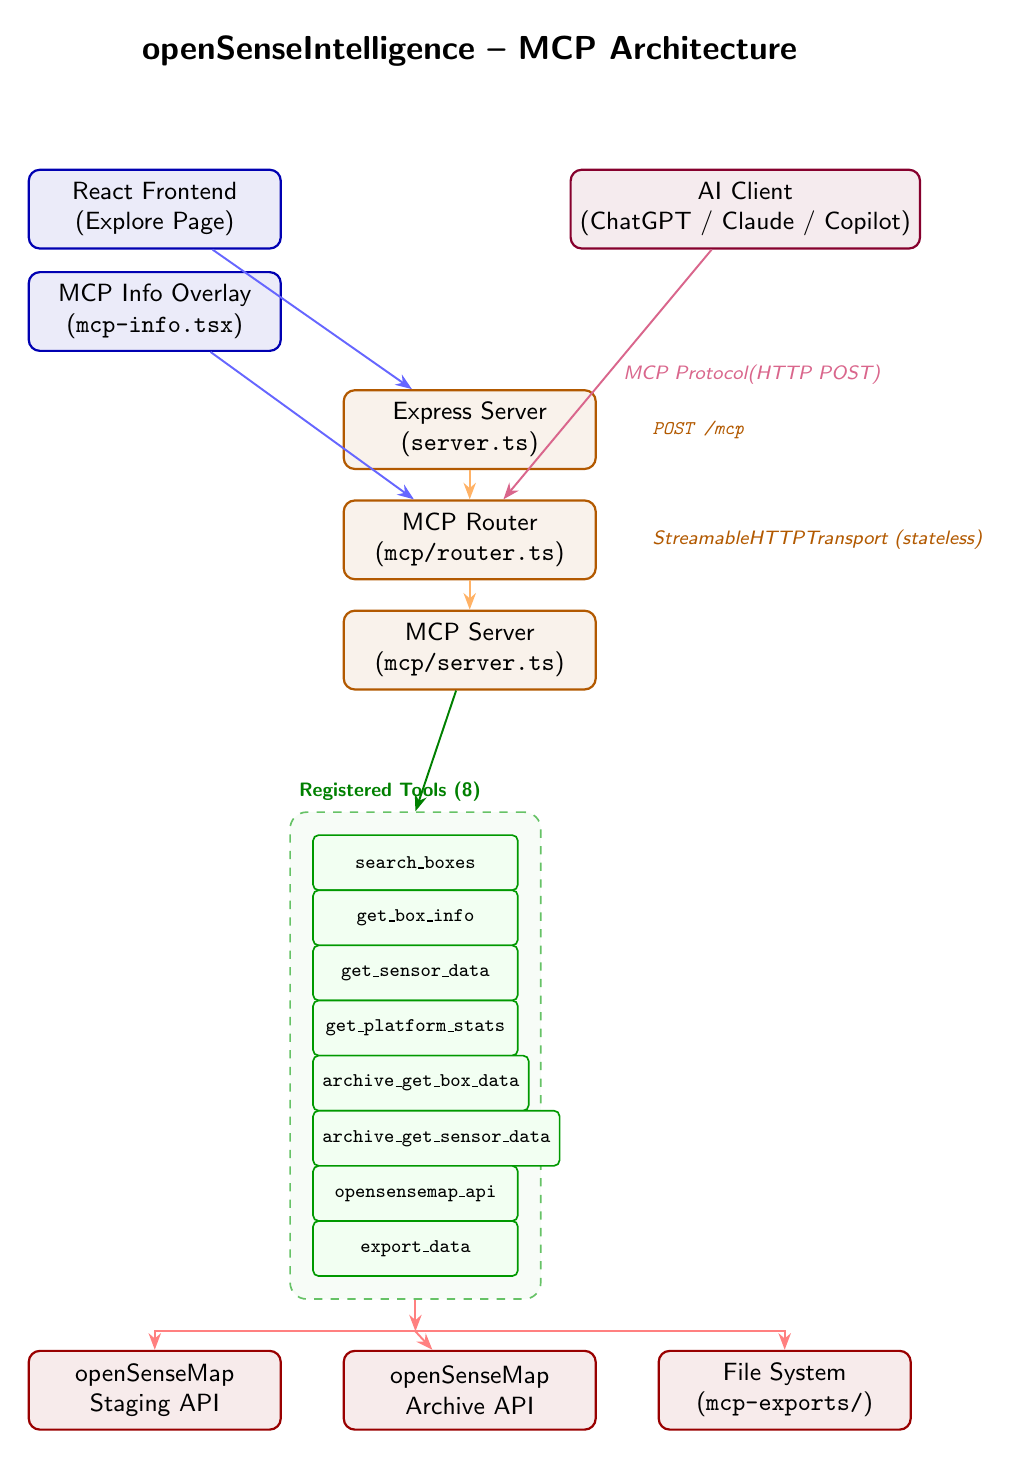
\begin{tikzpicture}[
    % Styles
    component/.style={
        rectangle, rounded corners=4pt, draw=#1, fill=#1!8,
        minimum width=3.2cm, minimum height=1cm,
        font=\small\sffamily, align=center, line width=0.8pt
    },
    component/.default=black,
    tool/.style={
        rectangle, rounded corners=2pt, draw=green!60!black, fill=green!5,
        minimum width=2.6cm, minimum height=0.7cm,
        font=\scriptsize\sffamily\ttfamily, align=center, line width=0.6pt
    },
    layer/.style={
        rectangle, rounded corners=6pt, draw=#1!60, fill=#1!3,
        line width=0.6pt, dashed
    },
    layer/.default=gray,
    arrow/.style={
        -{Stealth[length=6pt]}, line width=0.7pt, #1
    },
    arrow/.default=black!70,
    annot/.style={
        font=\scriptsize\sffamily\itshape, text=#1
    },
    annot/.default=black!60,
    title/.style={
        font=\large\sffamily\bfseries
    },
    subtitle/.style={
        font=\small\sffamily, text=black!60
    }
]

% Title
\node[title] at (0, 8.5) {openSenseIntelligence -- MCP Architecture};

% ── Frontend Layer ──────────────────────────────────────────────────────────
\node[component=blue!70!black] (frontend) at (-4, 6.5) {React Frontend\\(Explore Page)};
\node[component=blue!70!black] (mcpoverlay) at (-4, 5.2) {MCP Info Overlay\\(\texttt{mcp-info.tsx})};

% ── AI Client Layer ─────────────────────────────────────────────────────────
\node[component=purple!70!black] (aiclient) at (3.5, 6.5) {AI Client\\(ChatGPT / Claude / Copilot)};

% ── Express Server Layer ────────────────────────────────────────────────────
\begin{scope}[shift={(0, 2.5)}]
    \node[component=orange!70!black] (express) at (0, 1.2) {Express Server\\(\texttt{server.ts})};
    \node[component=orange!70!black] (mcprouter) at (0, -0.2) {MCP Router\\(\texttt{mcp/router.ts})};
    \node[component=orange!70!black] (mcpserver) at (0, -1.6) {MCP Server\\(\texttt{mcp/server.ts})};
    
    % Route labels
    \node[annot=orange!70!black, anchor=west] at (2.2, 1.2) {\texttt{POST /mcp}};
    \node[annot=orange!70!black, anchor=west] at (2.2, -0.2) {StreamableHTTP\\Transport (stateless)};
\end{scope}

% ── Tools Layer ─────────────────────────────────────────────────────────────
\node[tool, anchor=west] (t1) at (-2, -1.8) {search\_boxes};
\node[tool, anchor=west] (t2) at (-2, -2.5) {get\_box\_info};
\node[tool, anchor=west] (t3) at (-2, -3.2) {get\_sensor\_data};
\node[tool, anchor=west] (t4) at (-2, -3.9) {get\_platform\_stats};
\node[tool, anchor=west] (t5) at (-2, -4.6) {archive\_get\_box\_data};
\node[tool, anchor=west] (t6) at (-2, -5.3) {archive\_get\_sensor\_data};
\node[tool, anchor=west] (t7) at (-2, -6.0) {opensensemap\_api};
\node[tool, anchor=west] (t8) at (-2, -6.7) {export\_data};

\begin{pgfonlayer}{background}
    \node[layer=green!60!black, fit=(t1)(t8), inner sep=8pt] (toolbox) {};
\end{pgfonlayer}
\node[font=\scriptsize\sffamily\bfseries, text=green!50!black, anchor=south west] at (toolbox.north west) {Registered Tools (8)};

% ── External APIs ──────────────────────────────────────────────────────────
\node[component=red!60!black] (stagingapi) at (-4, -8.5) {openSenseMap\\Staging API};
\node[component=red!60!black] (archiveapi) at (0, -8.5) {openSenseMap\\Archive API};
\node[component=red!60!black] (filesystem) at (4, -8.5) {File System\\(\texttt{mcp-exports/})};

% ── Arrows ──────────────────────────────────────────────────────────────────

% Frontend → Server
\draw[arrow=blue!60] (frontend) -- (express);
\draw[arrow=blue!60] (mcpoverlay) -- (mcprouter);

% AI Client → MCP Router
\draw[arrow=purple!60] (aiclient) -- node[right, font=\scriptsize\sffamily\itshape, text=purple!60, xshift=2pt] {MCP Protocol\\(HTTP POST)} (mcprouter);

% Express → Router → Server
\draw[arrow=orange!60] (express) -- (mcprouter);
\draw[arrow=orange!60] (mcprouter) -- (mcpserver);

% Server → Tools
\draw[arrow=green!50!black] (mcpserver) -- (toolbox.north);

% Tools → External APIs
\draw[arrow=red!50] (toolbox.south) -- ++(0, -0.4) coordinate (apisplit);
\draw[arrow=red!50] (apisplit) -| (stagingapi);
\draw[arrow=red!50] (apisplit) -- (archiveapi);
\draw[arrow=red!50] (apisplit) -| (filesystem);

\end{tikzpicture}

\end{document}
